\documentclass[12pt]{article}
\usepackage{ctex}
\usepackage[english]{babel}
\usepackage{blindtext}
\usepackage{nameref}
\usepackage{fancyhdr}
\usepackage{amsmath,amssymb,amsthm}
\usepackage{graphicx,float}
\usepackage{physics}
\usepackage{pgfplots}
\usepackage[a4paper, total={6in, 9in}]{geometry}

\graphicspath{{../image/}}

\pagestyle{fancy}
\fancyhf{}
\fancyhf[HL]{極限}
\fancyhf[CF]{\thepage}

\newcommand{\innerprod}[2]{\langle{#1},{#2}\rangle}
\newcommand{\id}{\mathtt{id}}

\newtheorem{definition}{定義}
\newtheorem*{theorem}{定理}
\newtheorem*{corollary}{衍理}
\newtheorem*{lemma}{引理}
\newtheorem*{proposition}{設理}
\newtheorem*{remark}{小記}
\newtheorem*{claim}{主張}
\newtheorem*{example}{例子}
\newtheorem*{axiom}{公設}
\renewenvironment*{proof}{\textit{證明.}}{\hfill$\qed$}

\newenvironment*{sol}{\par \textbf{解}.}{\hfill$\blacksquare$}

\begin{document}
    \section*{無窮小量與無窮大量}
    
    在高等數學,對於無窮的討論,一般從無窮小量開始。何爲無窮小量?即一個非常接近0的變量不斷向零靠近,而永遠無法到達0,即爲無窮小量。

    我們可以考慮數列$\{a_n\}$, 其中對於任意整數$n$,$a_n=\dfrac{1}{10^n}$。則當$n$越大時,$a_n$越靠近0。對此,記$$a_n\to 0$$考慮對任意$n$,均有$\varepsilon>0$使得$0<\varepsilon<a_n$,則稱變量$\varepsilon$為無窮小量。記$\varepsilon\to 0$。

    相對的,考慮數列$\{A_n\}$, 其中對於任意整數$n$,$A_n=10^n$。則當$n$越大時,$A_n$越靠近$\infty$。對此,記$$A_n\to \infty$$考慮對任意$n$,均有$N>0$使得$A_n<N$,則稱變量$N$為無窮大量。記$N\to \infty$。

    由此發現,無窮小量與無窮大量互相關聯:

    \begin{axiom}
        若$a_n=\dfrac{1}{A_n}$,則$$\lim_{A_n\to \infty}a_n=0$$ 
    \end{axiom}

    以上亦可簡記為$\displaystyle\lim_{x\to\infty}\frac{1}{x}=0$.

    \section*{極限的幾何概念}

    想象一個漩渦,然後有一個點$p$在漩渦裏漂浮,其結果就是\textbf{$p$會不斷沿著漩渦中心繞圈,無限接近漩渦中心,但永遠不會到達中心}。此刻,我們稱$p$所走的路綫為$p$的\textbf{軌跡},記$p(t)$並以$t>0$作時間變數,而漩渦中心$p_0$則爲$p$的軌跡的極限,記$$p_0=\lim_{t\to\infty}p(t)$$

    \begin{figure}[H]
        \centering
        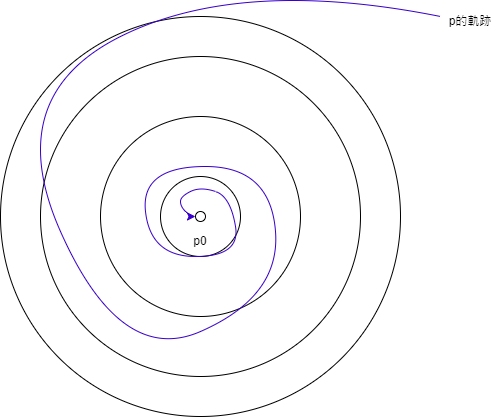
\includegraphics[scale=0.4]{limit1.png}
    \end{figure}    

    留意上圖,$p$的軌跡從外圍開始,不斷趨近於$p_0$。可見對於任何圓心為$p_0$且半徑爲$r>0$的圓形,均有$p(t)$位於圓形内。

    \section*{$\varepsilon-\delta$定義-於無窮小的極限}
    \section*{極限的性質}
    \section*{特殊的極限}
    \section*{於無窮大的極限}
    \section*{連續函數}
    \section*{連續函數的性質}
    \section*{介值定理}
    \section*{單調函數與逆函數}
\end{document}